\section{Связность и линейная связность}
\subsection{Связность}
% \begin{definition}[Связность]
% 	Топологическое пространство \(X\) называется связным, если его нельзя разбить на два непустых открытых множества:
% 	\begin{equation*}
% 		\forall U, V \open X: \ U \cap V = \varnothing \Rightarrow X \neq U \cup V.
% 	\end{equation*}
% \end{definition}
% \begin{statement}[Эквивалетное определение]
% 	Можно задать связности следующим образом:
% 	\begin{enumerate}
% 		\item \(\forall U, V \closed X: \ U \cap V = \varnothing \Rightarrow X \neq U \cup V\)
% 		\item \(\not\exists U\neq \varnothing\  \text{или} \ U = X : \ U \open X \ \text{и} \ U \closed X\)
% 	\end{enumerate}
% \end{statement}
% \begin{proof}
% 	Упражнение.
% \end{proof}


% \begin{example}
% 	\begin{enumerate}
% 		\item \textbf{Вещественная прямая} \( \mathbb{R} \) с обычной топологией является связным пространством.
		
% 		\item \textbf{Замкнутый интервал} \( [a, b] \) в \(\mathbb{R}\) также является связным пространством.
				
% 		\item \textbf{Окружность} \( S^1 \) в \(\mathbb{R}^2\) с обычной топологией также является связным пространством.
% 	\end{enumerate}
% \end{example}


% \begin{statement}[Непрерывный образ связного пространства]
% 	Пусть \( T_1 \) и \( T_2 \) являются топологическими пространствами и \( S_1 \subseteq T_1 \) является связным. Если \( f : T_1 \rightarrow T_2 \) является непрерывным отображением, тогда образ \( f(S_1) \) является связным.
% \end{statement}
% \begin{proof}
% 	Известно, что \( f : T_1 \rightarrow T_2 \). Пусть \(f(S_1) = U \sqcup V\), тогда \(S_1 = f^{-1}(U) \sqcup f^{-1}(V)\). Противоречие.
% \end{proof}

% \begin{corollary}[о промежуточных значениях]
% 	\(f\) принимает все промежуточные значения между инфимумом и супремумом.
% \end{corollary}



Связность — одно из фундаментальных свойств топологических пространств, которое позволяет описать их "целостность". Интуитивно, связное пространство — это такое пространство, которое нельзя разбить на две непересекающиеся части, каждая из которых является открытой. Это свойство играет ключевую роль в анализе, геометрии и физике, например, при изучении непрерывных процессов или путей в пространстве.

\begin{definition}[Связность]
Топологическое пространство $ X $ называется \textit{связным}, если его нельзя разбить на два непустых открытых множества:
\[
\forall U, V \subset X: \ U \cap V = \varnothing \Rightarrow X \neq U \cup V.
\]
Другими словами, не существует двух непустых открытых множеств $ U $ и $ V $, таких что $ X = U \cup V $ и $ U \cap V = \varnothing $.
\end{definition}

Связность можно определить несколькими эквивалентными способами. Эти формулировки полезны для доказательства различных свойств связных пространств.

\begin{statement}[Эквивалентные определения]
Следующие утверждения эквивалентны:
\begin{enumerate}
    \item Пространство $ X $ нельзя разбить на два непустых замкнутых множества:
    \[
    \forall U, V \closed X: \ U \cap V = \varnothing \Rightarrow X \neq U \cup V.
    \]
    \item Не существует нетривиального подмножества $ U \subset X $, которое одновременно открыто и замкнуто ($ U \neq \varnothing $ и $ U \neq X $).
\end{enumerate}
\end{statement}


Рассмотрим несколько примеров связных пространств, чтобы лучше понять это понятие.

\begin{example}
\begin{enumerate}
    \item \textbf{Вещественная прямая} $ \mathbb{R} $ с обычной топологией является связным пространством. Любая попытка разделить $ \mathbb{R} $ на два непересекающихся открытых множества приводит к противоречию.
    
    \item \textbf{Замкнутый интервал} $ [a, b] \subset \mathbb{R} $ также является связным. Например, если бы $ [a, b] $ можно было разбить на два непересекающихся открытых множества, то существовало бы "разрыв" между ними, что противоречит непрерывности интервала.
    
    \item \textbf{Окружность} $ S^1 \subset \mathbb{R}^2 $ с обычной топологией также является связным пространством. Окружность нельзя разделить на две непересекающиеся открытые части.
\end{enumerate}
\end{example}

Одно из важнейших свойств связности заключается в том, что она сохраняется при непрерывных отображениях. Это свойство широко используется в математическом анализе и топологии.

\begin{statement}[Непрерывный образ связного пространства]
Пусть $ T_1 $ и $ T_2 $ — топологические пространства, и пусть $ S_1 \subseteq T_1 $ является связным. Если $ f : T_1 \to T_2 $ — непрерывное отображение, то образ $ f(S_1) $ также является связным.
\end{statement}

\begin{proof}
Предположим, что $ f(S_1) $ можно разбить на два непересекающихся открытых множества $ U $ и $ V $, то есть $ f(S_1) = U \sqcup V $. Тогда прообразы $ f^{-1}(U) $ и $ f^{-1}(V) $ образуют разбиение $ S_1 $ на два непересекающихся открытых множества, что противоречит связности $ S_1 $.
\end{proof}


Свойство сохранения связности при непрерывных отображениях можно наглядно представить с помощью коммутативной диаграммы:

\[
\begin{tikzcd}[row sep=40pt, column sep=60pt]
    S_1 \arrow{r}{f} \arrow{d}{\text{связное}} & f(S_1) \arrow{d}{\text{связное}} \\
    T_1 \arrow{r}{f} & T_2
\end{tikzcd}
\]


Одним из важных следствий свойства связности является теорема о промежуточных значениях.

\begin{corollary}[Теорема о промежуточных значениях]
Если $ f : [a, b] \to \mathbb{R} $ — непрерывная функция, то $ f $ принимает все значения между $ \inf f $ и $ \sup f $.
\end{corollary}

\begin{proof}
Образ $ f([a, b]) $ связен, так как $ [a, b] $ связен и $ f $ непрерывно. Связное подмножество $ \mathbb{R} $ является интервалом, а значит, $ f $ принимает все промежуточные значения.
\end{proof}


% \begin{definition}[Компоненты связности]
% 	Компоненты связности -- это максимальные по включению связные подмножества пространства \(X\), такие что никакие два из них не пересекаются.
% \end{definition}

% \begin{example}
% 	\begin{enumerate}
% 		\item \textbf{Разрывная прямая:}
		
% 		Рассмотрим топологическое пространство \( X = [0,1] \cup [2,3] \subset \mathbb{R} \) с обычной топологией. Его компонентами связности являются отрезок \( [0,1] \) и отрезок \( [2,3] \).
		
% 		\item \textbf{Кольцо:}
		
% 		Пусть \( X = S^1 \times [0,1] \), где \( S^1 \) -- единичная окружность в плоскости, а \( [0,1] \) -- отрезок с обычной топологией. Тогда компонентами связности пространства \( X \) будут открытые диски, целиком содержащиеся внутри кольца \( S^1 \times (0,1) \).
		
% 		\item \textbf{Бесконечная лесенка:}
		
% 		Рассмотрим бесконечную лесенку \( X \) на плоскости, состоящую из счетного числа ступенек. Компонентами связности этой лесенки будут бесконечные лучи, выходящие из начальной точки и проходящие через каждую ступеньку.
% 	\end{enumerate}
% \end{example}

% \begin{statement}[о разбиение пространсва на компоненты связности]
% 	Каждое пространство разбивается на непересекающиеся компоненты связности.
% \end{statement}
% \begin{proof}
% 	Пусть \(x \in X\), рассмотрим \(Y = \bigcup_{x \in Y_x} Y_x\) -- компоненты связности в \(X\). Пусть \(Y_1, Y_2\) -- две различные компоненты связности, пусть \(x \in Y_1, Y_2\), тогда \(Y_1 \cup Y_2 = Y_1 = Y_2\).
% \end{proof}


% \begin{statement}
% 	Замыкание связного пространства -- связно.
% \end{statement}
% \begin{proof}
% 	Пусть \(Y\) -- связное пространство, тогда рассмотрим \(\mathrm{Cl}(Y)\), пусть \(\mathrm{Cl}(Y) = C \sqcup Z\), тогда \(Y \subseteq C\), следовательно \(\mathrm{Cl}(Y) \subseteq C\), отсюда \(Z = \varnothing\).
% \end{proof}

% \begin{corollary}
% 	Компоненты связности замкнуты.
% \end{corollary}
% \begin{proof}
% 	Пусть \(Y\) -- компонента связности, тогда \(\mathrm{Cl}(Y)\) -- связно, отсюда \(Y \subseteq \mathrm{Cl}(Y)\).
% \end{proof}


Компоненты связности — это максимальные связные подмножества топологического пространства. Они позволяют разбить пространство на "целостные" части, каждая из которых сама по себе является связной. Это свойство особенно полезно при анализе структуры сложных пространств, таких как разрывные множества или многообразия с особенностями.

\begin{definition}[Компоненты связности]
\textbf{Компоненты связности} — это максимальные по включению связные подмножества пространства $ X $, такие что никакие два из них не пересекаются.
\end{definition}

\begin{example}
\begin{enumerate}
    \item \textbf{Разрывная прямая:}
    
    Рассмотрим топологическое пространство $ X = [0,1] \cup [2,3] \subset \mathbb{R} $ с обычной топологией. Компонентами связности этого пространства являются отрезки $ [0,1] $ и $ [2,3] $. Эти отрезки не пересекаются и не могут быть объединены в одно связное множество.
    
    \begin{center}
        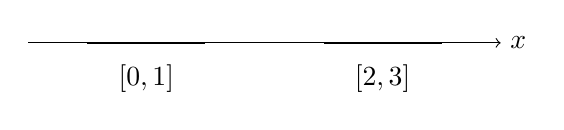
\begin{tikzpicture}[scale=1.5]
            % Оси
            \draw[->] (-0.5, 0) -- (3.5, 0) node[right] {$x$};
            
            % Отрезки
            \draw[thick] (0, 0) -- (1, 0);
            \draw[thick] (2, 0) -- (3, 0);
            
            % Подписи
            \node at (0.5, -0.3) {$[0,1]$};
            \node at (2.5, -0.3) {$[2,3]$};
            
        \end{tikzpicture}
    \end{center}

    \item \textbf{Кольцо:}
    
    Пусть $ X = S^1 \times [0,1] $, где $ S^1 $ — единичная окружность в плоскости, а $ [0,1] $ — отрезок с обычной топологией. Компонентами связности пространства $ X $ будут открытые диски, целиком содержащиеся внутри кольца $ S^1 \times (0,1) $.

    \item \textbf{Бесконечная лесенка:}
    
    Рассмотрим бесконечную лесенку $ X $ на плоскости, состоящую из счетного числа ступенек. Компонентами связности этой лесенки будут бесконечные лучи, выходящие из начальной точки и проходящие через каждую ступеньку.
\end{enumerate}
\end{example}

Одним из ключевых свойств компонент связности является то, что они образуют разбиение пространства.

\begin{statement}[О разбиении пространства на компоненты связности]
Каждое топологическое пространство разбивается на непересекающиеся компоненты связности.
\end{statement}

\begin{proof}
Пусть $ x \in X $. Рассмотрим $ Y_x $ — объединение всех связных подмножеств, содержащих точку $ x $. Покажите, что $ Y_x $ является связным и максимальным по включению. Если две компоненты связности пересекаются, то их объединение также связно, что противоречит максимальности.
\end{proof}


Еще одно важное свойство связности связано с замыканием множеств.

\begin{statement}[Замыкание связного пространства]
Замыкание связного пространства является связным.
\end{statement}

\begin{proof}
Пусть $ Y $ — связное пространство. Предположим, что $ \mathrm{Cl}(Y) $ можно разбить на два непересекающихся замкнутых множества $ C $ и $ Z $. Тогда $ Y \subseteq C $, и следовательно, $ \mathrm{Cl}(Y) \subseteq C $, что означает $ Z = \varnothing $.
\end{proof}


\begin{corollary}
Компоненты связности замкнуты.
\end{corollary}

\begin{proof}
Пусть $ Y $ — компонента связности. Поскольку $ \mathrm{Cl}(Y) $ связно и содержит $ Y $, то $ Y = \mathrm{Cl}(Y) $, то есть $ Y $ замкнуто.
\end{proof}

Свойства компонент связности можно наглядно представить с помощью коммутативной диаграммы:

\[
\begin{tikzcd}[row sep=40pt, column sep=60pt]
    X \arrow{r}{\text{разбиение}} \arrow{d}{\mathrm{Cl}} & \{Y_\alpha\} \arrow[d, closed hook arrow] \\
    \mathrm{Cl}(X) \arrow{r}{\text{разбиение}} & \{\mathrm{Cl}(Y_\alpha)\}
\end{tikzcd}
\]


\subsection{Линейная связность}

Линейная связность — это свойство топологического пространства, которое означает, что любые две точки в пространстве можно соединить непрерывным путем. Это свойство играет ключевую роль в анализе, геометрии и физике, например, при изучении непрерывных процессов или путей в пространстве. Линейно связные пространства часто возникают в задачах, связанных с движением частиц, деформациями объектов или потоками жидкости.

\begin{definition}[Линейная связность]
Топологическое пространство $ X $ называется \textbf{линейно связным}, если для любых двух точек $ x, y \in X $ существует непрерывная функция $ f: [0,1] \to X $, такая что:
\[
f(0) = x \quad \text{и} \quad f(1) = y.
\]
Функция $ f $ называется \textbf{путем}, соединяющим точки $ x $ и $ y $.
\end{definition}


Рассмотрим несколько примеров линейно связных пространств, чтобы лучше понять это понятие.

\begin{example}
\begin{enumerate}
    \item \textbf{Отрезок} $ [a, b] $ на вещественной прямой с обычной топологией является линейно связным. Любой путь между двумя точками можно задать как линейную интерполяцию:
    \[
    f(t) = (1-t)a + tb, \quad t \in [0,1].
    \]

    \item \textbf{Единичный круг} $ S^1 = \{(x, y) \in \mathbb{R}^2 \mid x^2 + y^2 = 1\} $ в плоскости также является линейно связным. Путь между двумя точками можно задать как дугу окружности.

    \item \textbf{Выпуклое множество}:
    Множество $ X \subset \mathbb{R}^n $ называется выпуклым, если для любых двух точек $ x_1, x_2 \in X $ и любого числа $ t \in [0,1] $ точка $ tx_1 + (1-t)x_2 $ также принадлежит множеству $ X $. Выпуклые множества всегда линейно связны, так как путь между любыми двумя точками можно задать как отрезок прямой.

    \begin{center}
		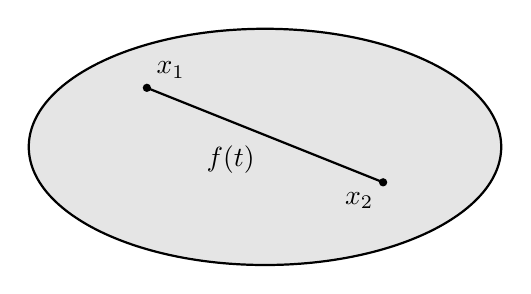
\begin{tikzpicture}[scale=1.5]
			% Выпуклое множество (штриховка)
			\draw[thick, fill=black!10] (0, 0) ellipse (2 and 1);
			
			% Две точки с метками
			\fill[black] (-1, 0.5) circle (1pt) node[above right] {$x_1$};
			\fill[black] (1, -0.3) circle (1pt) node[below left] {$x_2$};
			
			% Путь между точками
			\draw[thick] (-1, 0.5) -- (1, -0.3) node[midway, below left] {$f(t)$};
		\end{tikzpicture}
	\end{center}
\end{enumerate}
\end{example}


\begin{definition}[Компоненты линейной связности]
Компоненты линейной связности — это максимальные по включению линейно связные подмножества топологического пространства.
\end{definition}

Компоненты линейной связности можно рассматривать как "части" пространства, которые можно обойти, не покидая их. Например, если пространство состоит из нескольких разрозненных кусков, каждый кусок будет своей компонентой линейной связности.



Рассмотрим пример так называемого \textbf{топологического косинуса}. Это пространство показывает, что связность и линейная связность — это разные понятия.

\begin{example}[Топологический косинус]
Пусть $ X = \{ (x, \cos(1/x)) \mid x > 0 \} \cup \{ (0, y) \mid -1 \leq y \leq 1 \} $ — подмножество плоскости $ \mathbb{R}^2 $.

\begin{center}
    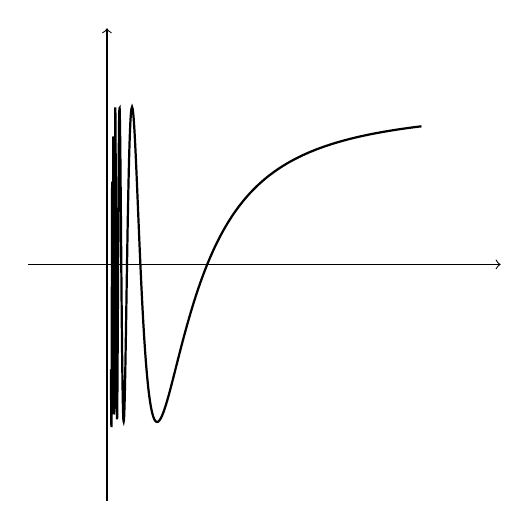
\begin{tikzpicture}[scale=2]
        % Ось Y
        \draw[->] (0, -1.5) -- (0, 1.5);
        
        % Ось X
        \draw[->] (-0.5, 0) -- (2.5, 0);
        
        % График cos(1/x)
        \draw[thick, domain=0.025:2, samples=500, smooth] plot (\x, {cos(1/\x r)});
        
        % Вертикальный отрезок
        \draw[thick] (0, -1) -- (0, 1);
	\end{tikzpicture}
\end{center}

Покажем, что точка $ (0,0) $ не соединяется путем с другими точками множества $ X $.

\begin{proof}
Пусть $ \gamma : [0,1] \to X $ — путь с началом в $ (0,0) $, то есть $ \gamma(0) = (0,0) $. Рассмотрим множество:
\[
T = \{ t \in [0,1] \mid \gamma(t) = (0,0) \}.
\]
Очевидно, что $ T $ замкнуто в $ [0,1] $, так как прообраз замкнутого множества $ \{(0,0)\} $ под непрерывным отображением $ \gamma $ является замкнутым.

Докажем, что $ T $ также открыто. Пусть $ t_0 \in T $. По определению, $ \gamma(t_0) = (0,0) $. По непрерывности пути $ \gamma $, найдётся $ \delta > 0 $, такое что для всех $ t \in (t_0 - \delta, t_0 + \delta) $ выполнено $ |\gamma(t)| < 1 $. Покажем, что $ \gamma(t) = (0,0) $ для всех $ t \in (t_0 - \delta, t_0 + \delta) $.

Допустим противное: существует $ t_1 \in (t_0 - \delta, t_0 + \delta) $, для которого $ \gamma(t_1) \neq (0,0) $. Тогда $ \gamma(t_1) = (x_1, \cos(1/x_1)) $ для некоторого $ x_1 > 0 $. Обозначим через $ \gamma_1(t) $ первую координату пути $ \gamma(t) $. Так как $ \gamma_1(t_1) > 0 $, по непрерывности найдётся $ t_2 \in [t_0, t_1] $, такое что $ \gamma_1(t_2) = \frac{1}{2\pi n} $, где $ n \in \mathbb{N} $. Тогда:
\[
\gamma(t_2) = \left(\frac{1}{2\pi n}, \cos(2\pi n)\right) = \left(\frac{1}{2\pi n}, 1\right).
\]
Но это противоречит предположению, что $ |\gamma(t)| < 1 $ для всех $ t \in (t_0 - \delta, t_0 + \delta) $. Таким образом, $ \gamma(t) = (0,0) $ для всех $ t \in (t_0 - \delta, t_0 + \delta) $.

Итак, множество $ T $ одновременно открыто и замкнуто в отрезке $ [0,1] $. Поскольку отрезок $ [0,1] $ является связным, то $ T = [0,1] $. Следовательно, путь $ \gamma(t) $ является постоянным и равен $ (0,0) $ для всех $ t \in [0,1] $.

Точка $ (0,0) $ не соединяется путем с другими точками множества $ X $.
\end{proof}
\end{example}

\starsection{Задачи и упражнения}

\begin{task}[Связность произведения пространств]
Докажите, что если $\mathrm{X}$ и $\mathrm{Y}$ — связные топологические пространства, то их произведение $\mathrm{X} \times \mathrm{Y}$ также является связным.
\end{task}

\begin{task}[Связность факторгруппы]
Пусть $\mathrm{H}$ и $\mathrm{G}$ — топологические группы, причем $\mathrm{H} \trianglelefteq \mathrm{G}$. Докажите, что если $\mathrm{H}$ и $\mathrm{G}/\mathrm{H}$ связны, то $\mathrm{G}$ также связно.

\textbf{Пояснение:} 
Используйте свойство фактортопологии. Постройте непрерывное отображение $\mathrm{G} \to \mathrm{G}/\mathrm{H}$ и покажите, что связность $\mathrm{G}/\mathrm{H}$ и $\mathrm{H}$ влечет связность $\mathrm{G}$.
\end{task}

\begin{task}[Общая линейная группа над $\mathbb{R}$]
Рассмотрим общую линейную группу $\mathrm{GL}_n(\mathbb{R})$ как подмножество пространства матриц $\mathrm{M}_{n \times n}(\mathbb{R})$. Покажите, что:
\[
\mathrm{GL}_n(\mathbb{R}) \overset{\det}{\longrightarrow} \mathbb{R} \setminus \{0\}
\]
неограниченно и несвязно.

\textbf{Пояснение:} 
Множество $\mathrm{GL}_n(\mathbb{R})$ состоит из всех невырожденных матриц. Определитель разбивает это множество на две компоненты: $\det(\mathrm{A}) > 0$ и $\det(\mathrm{A}) < 0$. Эти компоненты не пересекаются, что доказывает несвязность.
\end{task}

\begin{task}[Связность общей линейной группы над $\mathbb{C}$]
Докажите, что $\mathrm{GL}_n(\mathbb{C})$ — линейно связное пространство.
\end{task}

\begin{task}[Ортогональная группа $\mathrm{O}_n(\mathbb{R})$]
Докажите, что множество ортогональных матриц $\mathrm{O}_n(\mathbb{R})$:
\begin{enumerate}
	\item Компактно.
	\item Несвязно.
	\item Замкнуто.
\end{enumerate}

\textbf{Пояснение:} 
Компактность следует из ограниченности и замкнутости множества $\mathrm{O}_n(\mathbb{R})$. Несвязность обусловлена тем, что $\mathrm{O}_n(\mathbb{R})$ разбивается на две компоненты: матрицы с $\det(\mathrm{A}) = 1$ и $\det(\mathrm{A}) = -1$.
\end{task}

\begin{task}[Специальная ортогональная группа $\mathrm{SO}_n(\mathbb{R})$]
Докажите, что $\mathrm{SO}_n(\mathbb{R})$ (ортогональные матрицы с $\det(\mathrm{A}) = 1$) является линейно связным подмножеством $\mathrm{O}_n(\mathbb{R})$.
\end{task}

\begin{task}[Компоненты связности $\mathrm{O}_n(\mathbb{R})$]
Докажите, что $\mathrm{O}_n(\mathbb{R}) = \mathrm{SO}_n(\mathbb{R}) \sqcup \mathrm{O}_n^{-}(\mathbb{R})$, где $\mathrm{O}_n^{-}(\mathbb{R})$ — множество ортогональных матриц с $\det(\mathrm{A}) = -1$. Покажите, что каждая компонента линейно связна.
\end{task}

\begin{task}[Специальная линейная группа $\mathrm{SL}_n(\mathbb{R})$]
Докажите, что $\mathrm{SL}_n(\mathbb{R}) = \{\mathrm{A} \in \mathrm{M}_{n \times n}(\mathbb{R}) \mid \det(\mathrm{A}) = 1\}$:
\begin{enumerate}
	\item Линейно связно.
	\item Неограниченно.
	\item Замкнуто.
\end{enumerate}

\textbf{Пояснение:} 
Линейная связность следует из того, что любую матрицу с $\det(\mathrm{A}) = 1$ можно деформировать в единичную матрицу. Неограниченность обусловлена тем, что элементы матрицы могут быть сколь угодно большими. Замкнутость следует из непрерывности определителя.
\end{task}